Finora abbiamo visto delle proprietà generiche dei nuclei e abbiamo considerato alcuni casi di decadimento ed interazioni. Per fare dei progressi possiamo studiare il sistema più semplice: \textbf{interazione tra due nucleoni}. Per poterle interpretare, bisogna introdurre dei concetti nuovi: \textbf{spin} che è il momento angolare intrinseco di una particella, \textbf{fermioni} e il principio di Pauli e la teoria di \textbf{scattering quantistico}.
\subsection{Spin}
Una particella può presentarsi con un momento angolare \textbf{intrinseco}: intuitivamente può venir visto come se la particella ruotasse su sè stessa (anche se dobbiamo lasciare questa spiegazione solo all'ambito divulgativo.) In realtà corrisponde ad un \textbf{grado di libertà interno} della particella. Corrisponde a come la funzione d'onda di questo grado di libertà interno cambia in seguito ad una rotazione. Oltre all'operatore di momento angolare orbitale L:
\begin{equation*}
    \mathbf{L}=\mathbf{r}\times\mathbf{p}=-i\hbar\mathbf{r}\times \nabla \qquad [L_i,L_j]=i\hbar\varepsilon_{ijk}L_k
\end{equation*}
$L^2$ può avere autovalori $l(l+1)\hbar^2$, con $l=0,1,2,3,...$. Dato un asse di riferimento (es. $z$), $L_z$ ha autovalori $m\hbar$ con $m=l,l-1,...,-l+1,-l$. Esistono gli operatori di innalzamento e abbassamento che alzano o abbassano l di uno:
\begin{equation*}
    L_\pm=L_x\pm iL_y
\end{equation*}
Compare un \textbf{operatore di spin}, corrispondente al momento angolare intrinseco:
\begin{equation*}
    \mathbf{S}\qquad [S_i,S_j]=i\hbar\varepsilon_{ijk}S_k \qquad [L_i,S_j]=0
\end{equation*}
Il momento angolare totale è dato da 
\begin{equation*}
    \mathbf{J}=\mathbf{L}+\mathbf{S}
\end{equation*}
L'autovalore di $S^2=s(s+1)\hbar^2$ e questo $s$ è una proprietà intrinseca della particella, al pari di carica e massa. Quindi se dico che l'elettrone ha un determinato valore di $s$ tutti avranno questo valore. Se consideriamo una particella in un potenziale centrale, la sua funzione d'onda sarà etichettata in base ai numeri quantici radiale, di momenti angolare orbitale e dall'autovalore $m_s$ e di $S_z$. Quindi posso scrivere $\psi_{n,l,m,m_s}(\mathbf{r})$ Siccome lo spin non dipende dalla posizione si può utilizzare una notazione vettoriale per fattorizzare questo grado di libertà interno. In pratica noi diciamo che la funzione d'onda che ha i nostri gradi di libertà ($n,l,m$) che fanno parte della parte orbitale e l'autovalore $m_s$ lo posso vedere come una parte orbitale che dipende solo dallo spazio e un vettore a tre componenti con i tre possibili stati in cui può essere la particella. Ad esempio $s=1$ può esistere in tre stati:
\begin{equation*}
    \psi_{n,l,m,1}(\mathbf{r})=\psi_{n,l,m}(\mathbf{r})\left(\begin{array}{@{}c@{}}
1 \\
0 \\
0
\end{array}\right) \text{ ,}\quad     \psi_{n,l,m,0}(\mathbf{r})=\psi_{n,l,m}(\mathbf{r})\left(\begin{array}{@{}c@{}}
0 \\
1 \\
0
\end{array}\right) \text{ ,}\quad     \psi_{n,l,m,-1}(\mathbf{r})=\psi_{n,l,m}(\mathbf{r})\left(\begin{array}{@{}c@{}}
0 \\
0 \\
1
\end{array}\right)
\end{equation*}
Quindi rappresento i tre possibili autostati dei tre valori possibili di momenti angolari spin come dei vettori a 3 componenti. 

N.B.: da qui in poi, parlando di momenti angolari, diremo in maniera impropria: che una particella ha spin $s$ se il suo atovalore di $S^2$ è $s(s+1)\hbar^2$ e, di conseguenza, $S_z$ può assumere valori da $-s\hbar$ a $s\hbar$. Inoltre, in generale, ometteremo di scrivere esplicitamente $\hbar$.
\subsection{Spin 1/2}
In che cosa differisce lo spin dal momento angolare orbitale che abbiamo visto? Allora se noi ci mettiamo su uno spazio tridimensionale della particella ci troviamo con un certo numero di gradi di libertà. Se andiamo nello spazio intrinseco delle particelle possiamo dire che questa particella ha una sola componente ($s=0$ e unico possibile valore di $m_s=0$). Però posso anche dire due componenti come gradi di libertà intrinseca. Questa cosa è possibile perchè considerando uno spazio bi-dimensionale, gli operatori $S_i=1/2\sigma_i$ dove le $\sigma_i$ sono le "matrici di Pauli.
\begin{equation*}
    \sigma_1 =
\begin{pmatrix}0&1\\1&0\end{pmatrix}, \qquad \sigma_2 =
\begin{pmatrix}0&-i\\i&0\end{pmatrix} ,\qquad \sigma_3 =
\begin{pmatrix}1&0\\0&-1\end{pmatrix} 
\end{equation*}
Queste matrici di pauli hanno la caratteristica tale che se considero gli operatori $S_i$ soddisfano le regole di commutazione del momento angolare:$[S_i,S_j]=i\varepsilon_{ijk}S_k$. $S^2$ ha autovalore $3/4$:
\begin{equation*}
    \mathbf{S}^2=S_1^2+S_2^2+S_3^2=\frac{1}{4}[\sigma^2_1+\sigma^2_2+\sigma^2_3]=\frac{1}{4}[I+I+I]=\frac{3}{4}I
\end{equation*} 
Dove la $I$ è la matrice identità. Mentre $S_3$ ha autovalori $\pm\frac{1}{2}$, hanno le proprietà degli operatori di un momento angolare $s=1/2$. Quindi mentre il momento angolare orbitale può assumere solo valori interi, lo spin di una particella può assumere valori \textbf{interi e semi-interi}. Vedremo che particelle con valori semi-interi si comportano in maniera differente rispetto a valori interi.
\subsection{Rotazioni: momento angolare orbitale}
 Ricordiamo che gli operatori di momento angolare sono i generatori delle rotazioni. Esempio: se consideriamo una rotazione di un angolo infinitemsimo $\delta \omega$ attorno all'asse $z$ significa che mescolo le componenti $x$ e $y$:
 \begin{equation*}
     \psi(x,y,z)\to\psi(x-y\delta \omega,y+x\delta \omega,z)
 \end{equation*}
 Posso fare un'espansione di Taylor

\begin{align*}
\approx & \psi(x, y, z) - y\delta\omega \frac{\partial}{\partial x}\psi(x, y, z) + x\delta\omega \frac{\partial}{\partial y}\psi(x, y, z) \\
= & \psi(x, y, z) - \frac{i}{\hbar} y\delta\omega \left(-i\hbar \frac{\partial}{\partial x}\right)\psi(x, y, z) + \frac{i}{\hbar} x\delta\omega \left(-i\hbar \frac{\partial}{\partial y}\right)\psi(x, y, z) \\
= & \psi(x, y, z) + \frac{i}{\hbar}\delta\omega(xp_y-yp_x)\psi(x, y, z)
\end{align*}
ed una rotazione finita di un angolo $\omega$ è data da:
\begin{equation*}
    \psi(x, y, z)\to\exp{\left(\frac{i}{\hbar}\omega L_z\right)}\psi(x, y, z)
\end{equation*}
\subsection{Rotazioni: spin 1/2}
Vediamo come si comporta una funzione d'onda per spin $1/2$. L'operatore di rotazione è dato da:
\begin{equation*}
    \exp{\left(i\omega S_z\right)}=\sum_{n=0}^{+\infty}\frac{1}{n!}(i\omega S_z)^n=\sum_{n=0}^{+\infty}\frac{1}{n!}\left(\frac{i\omega}{2} \begin{bmatrix}1&0\\0&-1\end{bmatrix}\right)^n
\end{equation*}
Le potenze pari di questa matrice sono le matrici identità mentre le potenze dispari sono la stessa identica matrice. Quindi:
\begin{equation*}
    \begin{bmatrix} \sum_{n=0}^{+\infty}\frac{1}{n!}(\frac{i\omega}{2})^n & 0 \\ 
 &  \\ 0 & 
\sum_{n=0}^{+\infty}\frac{1}{n!}(-\frac{i\omega}{2})^n\end{bmatrix} = \begin{bmatrix} \exp{\left(\frac{i\omega}{2}\right)} & 0 \\ 
 &  \\ 0 & 
\exp{\left(-\frac{i\omega}{2}\right)}\end{bmatrix}
\end{equation*}
Una funzione d'onda con $S_z=+1/2$:
\begin{equation*}
    \psi_{+1/2}=\left(\begin{array}{@{}c@{}}
1 \\
0
\end{array}\right) \text{applicando la rotazione } \to e^{\frac{i\omega}{2}} \psi_{+1/2}
\end{equation*}
Una funzione d'onda con $S_z=-1/2$: 
\begin{equation*}
    \psi_{+1/2}=\left(\begin{array}{@{}c@{}}
0 \\
1
\end{array}\right) \text{applicando la rotazione } \to e^{-\frac{i\omega}{2}} \psi_{-1/2}
\end{equation*}
Come le autofunzioni del momento angolare, che per una rotazione cambiano di una fase $m\omega$. Questa cosa succede nella stessa maniera. Le autofunzioni del momento angolare cambiano di una fase sempre uguale a $m\omega$ con $m=\pm 1/2$. La cosa strana però è questa, Faccio una rotazione di $360^\circ$ mi aspetto che torno nella stessa posizione di prima. Se abbiamo oggetti che hanno spin semi-intero torno al punto di partenza ma la funzione ha cambiato segno:
\begin{equation*}
    \text{per una rotazione di } 2\pi: \psi\to-\psi
\end{equation*}
\subsection{Fermioni e bosoni}
Il numero quantico di \textbf{spin} può assumere \textbf{valori interi o semi-interi}. Perciò classifichiamo le particelle in base a questa caratteristica. Le particelle con spin intero sono dette \textbf{bosoni} ad esempio il fotone ha $s=1$. Le particelle con spin semi-intero sono dette \textbf{fermioni} ad esempio l'elettrone, il protone e il neutrone hanno $s=1/2$. Abbiamo appena visto che per una rotazione di $2\pi$ i bosoni non cambiano, mentre i fermioni cambiano di segno. Una trattazione matematica consistente mette in evidenza un'altra differenza fondamentale nel caso un sistema contenga \textbf{particelle identiche}: se sono \textbf{bosoni}, la funzione d'onda globale deve risultare \textbf{simmetrica} per lo scambio di particelle. Se sono \textbf{fermioni}, la funzione d'onda globale deve risultare \textbf{anti-simmetrica} per lo scambio di particelle. Un corollario importante è \textbf{il principio di esclusione di Pauli}: \textbf{due fermioni identici non possono avere gli stessi numeri quantici}. Questo perchè se avessero gli stessi numeri quantici, se scambio la particella 1 e la particella 2, la funzione d'onda dopo lo scambio ottengo la stessa funzione di partenza e quindi avrei una configurazione simmetrica per scambio di particella. Ma nel caso di fermioni non posso averla e quindi due particelle fermioniche non possono avere tutti i numeri quantici uguali. (spoiler i fermioni fanno quello che vogliono, hanno tante altre proprietà)
\subsection{Momento magnetico}
%IMMAGINE io oi
\begin{figure}[htp!]
  \centering
  
\includegraphics[scale=0.6]{Lezione6/io.png}
  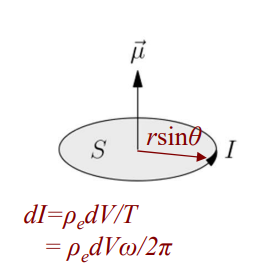
\includegraphics[scale=0.5]{Lezione6/oi.png} 
\end{figure}

Una particella può essere dotata di momento angolare: spin $\mathbf{S}$. In una visione classica, in cui una distribuzione di massa ruota con velocità angolare $\omega$ attorno al proprio asse:
\begin{equation*}
    \mathbf{S}=\int dV\rho(\mathbf{r})\mathbf{v}\times\mathbf{r} = \int dV\rho(\mathbf{r})(r\sin\theta\omega)(r\sin\theta)=\omega\int dV\rho(\mathbf{r})r^2\sin^2\theta=I\omega
\end{equation*}
con $I$ momento d'inerzia. Se abbiamo una corrispondente distribuzione di carica:
\begin{equation*}
    \rho_e(\mathbf{r})=\frac{Q}{M}\rho(\mathbf{r})
\end{equation*}
In questo caso la particella presenta anche un momento magnetico: sostanzialmente abbiamo che il volumetto infinitesimo percorre una circonferenza come se fosse della corrente che percorre una spira. E questa ha momento magnetico che è il valore della corrente moltiplicato per l'area della spira. La spira ha raggio $r\sin\theta$ e quindi ha area $\pi(r\sin\theta)^2$, e la corrente non è altro che la carica del mio volumetto diviso il tempo che impiega a percorrere il giro: $dI=\rho_edV/T=\rho_edV\omega/2\pi$. Quindi il momento angolare di un singolo volumetto è:
\begin{equation*}
    \mu=\int dV\rho_e(\mathbf{r})\frac{\nu}{2\pi r}(\pi r^2 \sin^2\theta)=\frac{Q}{2M}\omega\int dV\rho(\mathbf{r})r^2\sin^2\theta
\end{equation*}
dove il primo termine rappresenta la corrente e il secondo la superficie (prima della seconda uguaglianza). Quindi abbiamo che 
\begin{equation*}
    \mu=\frac{Q}{2M}S
\end{equation*}
Quindi in un sistema classico abbiamo una relazione ben definita tra momento angolare e momento magnetico generato dalla distribuzione di carica. Analogo, ma molto più complicato anche in un sistema quantistico. 

In meccanica quantistica solo alcuni valori di $\mathbf{S}$ sono permessi:
\begin{equation*}
    S=\sqrt{s(s+1)} \quad s=0,\frac{1}{2},1,\frac{3}{2},... \qquad S_z=m \quad m=-s,-s+1,...,+s
\end{equation*}
Il momento magnetico si può esprimere come
\begin{equation*}
    \Vec{\mu}=g\frac{Q\hbar}{2M}\mathbf{S}
\end{equation*}
dove $g$ è il fattore giromagnetico (non presente in meccanica classica). $p$,$n$ ed $e$ hanno tutti $s=1/2$ quindi possono trovarsi in due stati di $S_z=\pm\hbar/2$. Una trattazione relativistica (equazione di Dirac) dà che $g=2$ per particelle \textbf{elementari} di spin $1/2$. Prima differenza importante tra meccanica classica ($g=1$) e meccanica quantistica per particelle puntiformi senza nessun tipo di struttura interna ($g=2$). Per l'elettrone abbiamo che 
\begin{equation*}
    \mu_e=\mu_B=\frac{e\hbar}{2m_e}=5.788381\times10^{-11}\,MeV/T \qquad g_e\approx2
\end{equation*}
Detto \textbf{magnetone di Bohr}. Per il protone:
\begin{equation*}
    \mu_p=2.79\mu_N=2.79\frac{e\hbar}{2m_p}  \qquad g_p=5.58
\end{equation*}
dove $\mu_N=3.152451\times10^{-14}\,MeV/T$ è detto \textbf{magnetone nucleare}. Se fosse una particella elementare il fattore giromagnetico dovrebbe essere circa uguale a $2$ ma questo non succede infatti: $g_p=5.58$. Per il neutrone è ancora più "imbarazzante", classicamente, essendo neutro, mi viene in mente che il momento magnetico del neutrone dovrebbe essere nullo. In realtà si scopre essere:
\begin{equation*}
    \mu_n=-1.91\mu_N \qquad g_n=-3.82
\end{equation*}
è orientato in maniera opposta rispetto allo spin, e di conseguenza abbiamo che $g_n=-3.82$. Questa osservazione è un primo segnale che protone e neutrone non possono essere oggetti fondamentali rispetto alla meccanica quantistica. Perchè non ha le proprietà per cui possono essere riconosciute particelle elementari in meccanica quantistica. Se una particella è una particella puntiforme effettivamente non può avere momento magnetico. Questo succede effettivamente con il \textbf{fotone}. Mentre invece una particella composta anche se neutra globalmente può avere momento magnetico come abbiamo visto per il \textbf{neutrone}.
\subsection{Spin e momenti magnetici dei nuclei}
Essendo i nuclei costituiti da neutroni e protoni possono presentare un momento angolare dato dalla composizione degli spin e dei momenti angolari orbitali dei singoli protoni e neutroni. Ci riferiremo a questo momento angolare come \textbf{spin del nucleo}: $J$. Analogamente i momenti magnetici: intrinseci di $n$ e $p$ ed orbitali $\mu_N L$ (per la parte orbitale $g=1$ come ci aspettiamo in meccanica classica) però quando si combinano i momenti magnetici orbitali ($g=1$) con gli spin di neutrone e protone che hanno un fattore giromagnetico diverso da 1: \textbf{momento magnetico}: $\mu=g_J\,\mu_NJ$. Queste sono osservabili nelle interazioni con campi magnetici esterni: questo perchè l'energia di un dipolo in un campo magnetico è: $E=-\Vec{\mu}\cdot \mathbf{B}$. Questa energia si traduce nel fatto di avere $2j+1$ livelli energetici perchè a seconda della proiezione di $\mu$ lungo l'asse del campo magnetico posso avere diversi valori di questa energia scalati da $m_j$. $m_j$ è il momento angolare lungo l'asse $j$. $E=g_J\mu_NBm_j$ con $-j\le m_j\le j$. Quello che succede è che io posso misurare questo $g_J\mu_N$ perchè se io ho un campione di un materiale che è in un campo magnetico e io fornisco a questo campione energia (sottoforma di radiazione) ad una frequenza ben specifica che corrisponde a quanti di energia $h\nu$ avviene una transizione con l'assorbimento dei fotoni. Processo chiamato \textbf{risonanza magnetica nucleare} vedo che ho un assorbimento di energia da parte dei miei nuclei e se ho una radiazione elettromagnetica che è esattamente uguale alla differenza di energia del salto tra liveli effettuato $\Delta E=g_j\mu_nB$. In presenza di questi effetti la separazione delle traiettorie dipendono da $m_j$ perchè sentono delle forze diverse in base al gradiente del campo. 
\subsection{Scattering elettrone-nucleo(ne)}
Si sta parlando di un esperimento di Scattering fatto in maniera tale da mettere in evidenza la struttura all'interno del nucleo che Ruttherford non poteva vedere attraverso le particelle $\alpha$. Il metodo principe per farlo è sfruttare il processo di scattering usando gli elettroni. Si sta parlando di un processo elettromagnetico quindi non ci serve sapere come sono fatte le interazioni forti. Quindi riesco a studiare le varie interazioni proprio perchè utilizzo un elettrone e quindi ci sono in gioco solo fenomeni che si conoscono bene. 
\subsection{Scattering su potenziale fisso}
La \textbf{probabilità di transizione per unità di tempo} da uno stato iniziale $i$, ad uno stato finale $f$, causata dall'interazione con un potenziale $U$, è descritto dalla \textbf{regola d'oro di Fermi}. Questa regola arriva da un calcolo dalla teoria delle perturbazioni quantistiche. Che ci dice che se io ho dei atustati di un certo tipo di interazione e aggiungo una perturbazione cioè qualcosa che mi modifica i miei autostati allora a questo punto gli autostati del potenziale originale non sono più autostati del moto ma la mia funzione d'onda si può evolvere nel tempo e quindi cambiare forma. 
\begin{equation*}
    P={\frac {2\pi }{\hbar }}\left|\langle f|U|i\rangle \right|^{2}\rho (E_{f})
\end{equation*}
Dove compaiono:
\begin{itemize}
    \item l'elemento di matrice: $\langle f|U|i\rangle=\int d\mathbf{r}\psi^{*}_f(\mathbf{r})U(\mathbf{r})\psi_i(\mathbf{r})$ 
    \item le funzioni d'onda che compaiono in questo elemento di matriche sono della particella libera, normalizzate sul volume: $\psi(\mathbf{r})\propto\frac{1}{\sqrt{V}}e^{-i\mathbf{p}\cdot\mathbf{r}}$
\end{itemize}
Questo perchè visto che sto facendo un esperimento di scattering si guardano gli stati iniziali e finali molto lontani dal centro dell'interazione. Con i momenti (assumento che l'asse $z$ sia diretto lungo il moto delle particelle):
\begin{equation*}
    \mathbf{p}_i=p\left(\,0,\,0,\,1\,\right) \qquad \mathbf{p}_f=p\left(\;\sin\theta\cos\phi,\,\sin\theta\sin\phi,\,\cos\theta\,\right)
\end{equation*}
L'altro termine è la densità di stati finali: (spazio delle fasi) ovvero è il numero di stati finali in un certo intervallo infinitesimo di energia. Questo numero è:
\begin{equation*}
    \rho(E_f)=\frac{dN}{dE_f}=\frac{Vp_f^2d\Omega}{(2\pi\hbar)^3}\frac{dp_i}{dE_f}
\end{equation*}
Essendo una densità è il numero di stati per un'unità di energia, lo stato finale in questo caso è l'elettrone che esce dall'interazione con una cerca direzione e momento. La densità degli stati finali è definita in termini di numeri di stati presenti in un certo volume di spazio delle fasi (dato dallo spazio delle cordinate e dallo spazio dei momenti). In questo spazio delle fasi un elettrone che esce con una certa quantità di moto con un certo angolo solido occupa un volume nello spazio delle fasi sarà il volume fisico occupato moltiplicato per il volumetto nello spazio dei momenti $Vp^2_fd\Omega dp$ quindi un volumetto su una sfera di raggio $p_f$ e angolo solido $d\Omega$. Quindi $p_f^2 d\Omega$ è la superficie sottesa dall'angolo solido sulla sfera. Moltiplico per lo "spessore" $dp_f$ e trovo il volumetto infintesimo dello spazio delle fasi. Si può vedere che il volume occupato nello spazio delle fasi è circa proporzionale a $h$. Qui siamo in 3 dimensioni quindi $h^3$. Quindi:
\begin{equation*}
    dN=\frac{Vp_f^2d\Omega dp_f}{h^3}
\end{equation*}
Divido per $dE_f$ pechè è una densità di stati in funzione dell'energia.
Passando ora all'elemento di matrice:
\begin{equation*}
    \langle f|U|i\rangle=\int d\mathbf{r}\psi^*_f(\mathbf{r})U(\mathbf{r})\psi_i(\mathbf{r})=\int d\mathbf{r}\frac{1}{V}e^{i\mathbf{p}_f\cdot\mathbf{r}}U(\mathbf{r})e^{-i\mathbf{p}_i\cdot\mathbf{r}}=\frac{1}{V}\int d\mathbf{r}e^{-i(\mathbf{p}_i-\mathbf{p}_f)\cdot\mathbf{r}}U(\mathbf{r})
\end{equation*}
Ponendo $\mathbf{q}=\mathbf{p}_i-\mathbf{p}_f$, chiamato\textbf{ momento trasferito}, ottendo:
\begin{equation*}
    \langle f|U|i\rangle=\frac{1}{V}\int d\mathbf{r}U(\mathbf{r})e^{-i\mathbf{q}\cdot\mathbf{r}}=\frac{1}{V}\tilde{U}(\mathbf{q})
\end{equation*}
Quell'integrale non è altro che la trasformata di Fourier del potenziale valutata nel vettore $\mathbf{q}$. Questo $\mathbf{q}$ non è altro che:
\begin{equation*}
    \mathbf{q}=|\mathbf{p}|\left(\,-\sin\theta\cos\phi,\,-\sin\theta\sin\phi,\,1-\cos\theta\,\right)
\end{equation*}
Facendone il quadrato
\begin{equation*}
    \mathbf{q}^2=\mathbf{p}^22(1-\cos\theta)=\mathbf{p}^24\sin^2\theta/2
\end{equation*}
Nel caso di scattering su potenziale fisso, dato che energia iniziale e finale coincidono, $\mathbf{q}$ in pratica coincie con il \textbf{tetramomento trasferito}:
\begin{equation*}
    q=\left(\,0,\,\mathbf{q}\,\right) \qquad q^2=-\mathbf{q}^2
\end{equation*}

Quale è il legame tra questa regola d'oro di fermi e la sezione d'urto? Se pongo che $p_f=\sqrt{2mE_f}$, allora la probabilità di transizione per unità di tempo è:
\begin{equation*}
     P={\frac {2\pi }{\hbar }}\left|\langle f|U|i\rangle \right|^{2}\rho (E_{f})=2\pi\frac{\left|\tilde{U}(\mathbf{q})\right|^2}{V^2}\frac{V}{(2\pi)^3}\frac{p_f^2dp_f}{dE_f}d\Omega=\frac{1}{V}\frac{\left|\tilde{U}(\mathbf{q})\right|^2}{4\pi^2}\frac{p_f^2dp_f}{dE_f}d\Omega
\end{equation*}
Possiamo trovare una relazione tra questa probabilità di transizione per unità di tempo ed il tasso di interazioni dato dalla sezione d'urto:
\begin{equation*}
    \frac{dN}{dt}=In_Tdz\frac{d\sigma}{d\Omega}d\Omega
\end{equation*}
Questo è il punto importante perchè ci permette di collegare quello che possiamo calcolare teoricamente dato un potenziale e quello che possiamo misurare. Devo trovare il legame tra queste due grandezze. Nel nostro sistema, una sola particella che può cambiare stato quindi abbiamo che $dN/dt=P$. La corrente $I$ che abbiamo dentro la sezione d'urto è data dal rapporto del numero di particelle incidenti $(=1)$ e il tempo che le particelle impiegano ad attraversare il volume di interazione: $I=1/(dz/v_i)$. Abbiamo un solo bersagio nel volume: $n_T=1/V$ e quindi sostituendo ed eguagliando trovo:
\begin{equation*}
     P=v_i\frac{1}{V}\frac{d\sigma}{d\Omega}d\Omega
\end{equation*}
ed infine per scattering elastico, quindi si conserva la quantità di moto e l'energia cinetica:
\begin{equation*}
    \frac{d\sigma}{d\Omega}=\frac{\left|\tilde{U}(\mathbf{q})\right|^2}{4\pi^2}\frac{1}{v}\frac{p^2dp}{dE}
\end{equation*}
\textbf{La sezione d'urto differenziale che è una quantità che possiamo misurare ci da come informazione la trasformata di Fourier del potenziale di interazione.} Questo è il legame quantistico tra sezione d'urto e potenziale. Ovvero la sezione d'urto differenziale che è una quantità che possiamo misurare ci da come informazione la trasformata di Fourier del potenziale di interazione. Per cui se misuriamo la sezione d'urto otteniamo la trasformata di Furier del potenziale e calcolando l'antitrasformata possiamo calcolarci il potenziale. Viceversa se sappiamo come è fatto il potenziale possiamo calcolarci la sezione d'urto. Su questa identià si basano tutti i nostri esperimenti di scattering.
\subsubsection{Spazio delle fasi}
Il termine di spazio delle fasi $\rho(E_f)$ definisce il numero di stati disponibili $dN$ in un intervallo infinitesimo di energia:
\begin{equation*}
    dN=\rho(E_f)dE_f
\end{equation*}
è dato dal rapporto del volume nello spazio delle fasi (coordinate x momenti) e la costante di Plank $h$ (volume occupato da uno stato quantistico):
\begin{equation*}
    dN=\frac{dxdydzdp_xdp_ydp_z}{(2\pi\hbar)^3}
\end{equation*}
Nel caso specifico di una particella libera con un dato momento: La funzione d'onda occupa tutto il volume $V$, per cui possiamo integrare la componente spaziale del $dN$. Possiamo anche esprimere il differenziale in momento in termini delle coordinate polari, per evidenziare il modulo del momento $p_f$, correlato all'energia della particella, e la direzione nel termine di angolo solido $d\Omega$:
\begin{equation*}
    dN=\frac{Vp^2_fdp_fd\Omega}{(2\pi\hbar)^3}
\end{equation*}
\subsubsection{Fattore di forma}
Questo concetto è un modo per estrarre dalla trasformata di fourier la distribuzione di carica. Quello che vogliamo fare a livello sperimentale è andare a vedere la distribuzione di carica all'interno del nucleo. Nel caso di scattering su carica puntiforme dopo aver calcolato la trasformata di Fourier del potenziale coulombiano:
\begin{equation*}
    \tilde{U}_{punt.}(\mathbf{q})=\frac{e^2}{\varepsilon_0\mathbf{q}^2}=\frac{e^2}{4\varepsilon_0\mathbf{p}^2\sin^2\theta/2}
\end{equation*}
e la sezione d'urto differenziale (relativistica):
\begin{equation*}
    \frac{d\sigma}{d\Omega}=\frac{\alpha^2}{4E^2\sin^4\theta/2}
\end{equation*}
che rirpoduce quello che abbiamo visto con il calcolo classico. Consideriamo cosa succede quando il potenziale non è generato da una particella puntiforme ma generato da una \textbf{distribuzione di carica} generica con densità $\rho(\mathbf{r})$ normalizzata a $1$:
\begin{equation*}
    U(\mathbf{r})=\int d\mathbf{r}'\frac{e^2\rho(\mathbf{r}')}{4\pi\varepsilon_0|\mathbf{r}-\mathbf{r}'|}
\end{equation*}
\begin{equation*}
    \langle f|U|i\rangle=\frac{1}{V}\int d\mathbf{r}e^{i\mathbf{p}_f\cdot\mathbf{r}}\left[\int d\mathbf{r}'\frac{e^2\rho(\mathbf{r}')}{4\pi\varepsilon_0|\mathbf{r}-\mathbf{r}'|}\right]e^{-i\mathbf{p}_i\cdot\mathbf{r}}
\end{equation*}
E quindi:
\begin{equation*}
    \int d\mathbf{r}\int d\mathbf{r}'\frac{e^2\rho(\mathbf{r}')}{4\pi\varepsilon_0|\mathbf{r}-\mathbf{r}'|}e^{-i\mathbf{q}\cdot\mathbf{r}}=\ldots=\frac{e^2}{\varepsilon_0\mathbf{q}^2}\int d\mathbf{r}'\rho(\mathbf{r}')e^{-i\mathbf{q}\cdot\mathbf{r}'}
\end{equation*}
Ovvero 
\begin{equation*}
    \tilde{U}(\mathbf{q})=\tilde{U}_{punt.}(\mathbf{q})F(\mathbf{q})
\end{equation*}
E questo ci dice che la trasformata di Fourier del potenziale generato da una distribuzione di carica lo posso vedere come la trasformata di Fourier di una carica puntiforme moltiplicato per il \textbf{fattore di forma}:
\begin{equation*}
    F(\mathbf{q})=\int d\mathbf{r}\rho(\mathbf{r})e^{-i\mathbf{q}\cdot\mathbf{r}}
\end{equation*}
Per quanto riguarda l'interpretazione dei fattori di forma viene ereditata dalla meccanica quantistica dal fatto che gli oggetti che stiamo studiando non sono più puntiformi o rigidi ma delle onde di probabilità che creano interferenza. Se il processo di scattering avviene non in un punto, ma su una distribuzione di densità compare un contributo dovuto alla propagazione delle onde piane corrispondenti alle funzioni d’onda della particelle incidente e di quella
diffusa:
\begin{equation*}
    F(\mathbf{q})=\int d\mathbf{r}e^{i\mathbf{p}_f\cdot\mathbf{r}}\rho(\mathbf{r})e^{-i\mathbf{p}_i\cdot\mathbf{r}}=\int d\mathbf{r}e^{i\mathbf{q}\cdot\mathbf{r}}\rho(\mathbf{r})
\end{equation*}
Per particelle puntiformi:
\begin{equation*}
    \rho(\mathbf{r})=\delta(\mathbf{r})\,\Rightarrow\,F(\mathbf{q})=1
\end{equation*}
A basso momento trasferito cioè quando $q<<1/r$, sviluppando l'integrale si ottiene una serie di potenze in $\mathbf{q}$:
\begin{equation*}
    F(\mathbf{q})=\int d\mathbf{r}e^{i\mathbf{q}\cdot\mathbf{r}}\rho(\mathbf{r})=\int d\mathbf{r}\rho(\mathbf{r})\left[1+i\mathbf{q}\cdot\mathbf{r}-\frac{1}{2}\left(\mathbf{q}\cdot\mathbf{r}\right)^2+\ldots\right]
\end{equation*}
Assumento $\rho$ a simmetria sferica (che abbiamo visto essere una buona approssimazione visto che è una configurazione energeticamente favorita): $F(\mathbf{q})=F(q^2)$
\begin{equation*}
    \int d\mathbf{r}\rho(\mathbf{r})=1 \qquad \int d\mathbf{r}\rho(\mathbf{r})i\mathbf{q}\cdot\mathbf{r}=0
\end{equation*}
Dove il primo termine è uguale a uno per definizione mentre il secondo termine è una quantità dispari integrato in un dominio simmetrico e quindi deve fare $0$. Il terzo contributo:
\begin{equation*}
    -\frac{1}{2}\left(\mathbf{q}\cdot\mathbf{r}\right)^2=-\frac{1}{6}\mathbf{q}^2\left\langle r^2\right\rangle
\end{equation*}
In quanto questo integrale è circa uguale a calcolarsi il raggio quadratico medio. L'esperimento di Hofstadter è proprio andare a misurare questo terzo termine per ricavare $r^2$. 

Quindi se $q<<1/r$, l'integrale oscilla fortemente e $F(q^2)\to0$ per $\mathbf{q}^2\to\infty$. Infatti se penso alla particella puntiforme il \textbf{fattore di forma} è $1$. Per le distribuzione di carica questo contributo è $<1$ in quanto abbiamo visto che sviluppando l'esponenziale è negativo. Questa è una proprietà generale dei fattori di forma. Se ci ricordiamo questo torna con il fato che l'esperimento di Rutherford vedeva particelle $\alpha$ deviate di grande angolo e quindi grande $q^2$ (momento trasferito molto elevato). Il fatto che lo vedo significa che il fattore di forma deve essere per forza molto vicino a uno e quindi qualcosa di puntiformi secondo la scala dell'esperimento di Rutherford ma non nell'esperimento di Ofstadter.

\subsection{Cinematica}
Consideriamo un elettrone incidente su un nucleo a riposo dove:
%IMMAGINE dsds gg
\begin{figure}[htp!]
  \centering
  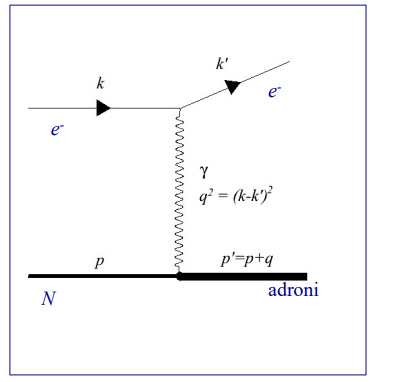
\includegraphics[scale=0.6]{Lezione6/dsds.png}
  
\includegraphics[scale=0.5]{Lezione6/gg.png} 
\end{figure}
\begin{itemize}
    \item $\mathbf{k}$ è il tetramomento iniziale dell'elettrone;
    \item $\mathbf{p}$ il tetramomento iniziale del nucleo;
    \item $\mathbf{k}'$ il tetramomento dell'elettrone dopo l'interazione;
    \item $\mathbf{q}$ il momento trasferito.
\end{itemize}
Per fissare le idee definiamo l'ase $z$ come la direzione del moto, possiamo trascurare la massa dell'elettrone (possiamo metterci a regime ultra-relativistico). Tra i due oggetti avviene un'interazione elettromagnetica. Quindi l'elettrone scambia un fotone con il nucleo, trasferendogli un tetramomento $\mathbf{q}$. Una variabile interessante è la massa dello stato adronico finale:
\begin{equation*}
    W^2=(p+q)^2=m_N^2+2(pq)+q^2
\end{equation*}
Ricordo che il quadrato di un tetramomento rappresenta una massa. Se il nucleo viene eccitato il sistema che viene creato globalmente lo possiamo vedere come una massa $W^2$.

Quindi ricapitolando abbiamo tre tetravettori indipendenti:$\mathbf{p},\mathbf{k},\mathbf{k'}$. Non è presente $\mathbf{p'}$ perchè lo posso ricavare dagli altri tre. Questi tre tetravettori possono venire combinati a dare tre quantità scalari. Ad esempio l'energia al quadrato del centro di massa:
\begin{equation*}
    s=(p+k)^2=m_N^2+2m_NE
\end{equation*}
E poi due a scelta tra \textbf{momento trasferito}:
\begin{equation*}
    q^2=(k-k')^2=-2(kk')=-2EE'(1-\cos{\theta})=-4EE'\sin^2{\frac{1}{2}\theta}
\end{equation*}
Per comodità si definisce $Q^2$ come quantità positiva: $Q^2=-q^2$.

\textbf{Frazione di energia trasferita}:
\begin{equation*}
    y=\frac{2(pq)}{2(pk)}=\frac{E-E'}{E} \qquad 0<y<1
\end{equation*}
Ed infine $\mathbf{x_B}$:
\begin{equation*}
    x=\frac{Q^2}{2(pq)} \qquad 0<x<1
\end{equation*}
Anche questo ultimo fattore è molto usato infatti nel \textbf{caso elastico} un vincolo aggiuntivo $W^2=m_N^2$. In questa situazione visto che $W^2=(p+q)^2=m_N^2+2(pq)+q^2$ la uguaglio con $m_N$:
\begin{equation*}
    m_N^2=m_N^2+2(pq)+q^2 \,\Rightarrow\,x=\frac{-q^2}{2(pq)}=1
\end{equation*}
e quindi:
\begin{equation*}
    \frac{-2EE'(1-\cos{\theta})}{2m_N(E-E')}=1 \quad \Rightarrow\quad\frac{E'}{E}=\frac{1}{1+(E/m_N)(1-\cos{\theta})}=\frac{1}{1+(2E/m_N)\sin^2{\frac{1}{2}\theta}}
\end{equation*}
\subsection{Sezioni d'urto di Mott e Dirac}
La sezione d'urto di\textbf{ Rutherford}:
\begin{equation*}
    \left(\frac{d\sigma}{d\Omega}\right)_\text{Rutherford}=\frac{\alpha^2}{4E^2\sin^2{\frac{1}{2}\theta}}
\end{equation*}
è stata calcolata senza tenere conto del contributo dovuto al momento magnetico dell'elettrone. Quando si considera lo spin dell'elettrone, la sezione d'urto di Rutherford viene modificata da un fattore puramente angolare e viene detta sezione d'urto di \textbf{Mott}:
\begin{equation*}
    \left(\frac{d\sigma}{d\Omega}\right)_\text{Mott}=\left(\frac{d\sigma}{d\Omega}\right)_\text{Rutherford}\cos^2{\frac{1}{2}\theta}
\end{equation*}
Ed è la sezione d'urto che consideriamo quando parliamo di diffusione degli elettroni. Se si considera un bersaglio puntiforme con spin $\frac{1}{2}$ (interazione tra due elettroni uno fermo e uno in movimento) abbiamo la sezione d'urto di \textbf{Dirac}:
\begin{equation*}
    \left(\frac{d\sigma}{d\Omega}\right)_\text{Dirac}=\left(\frac{d\sigma}{d\Omega}\right)_\text{Mott}\left[1+\frac{Q^2}{2m_N^2}\tan^2{\frac{1}{2}\theta}\right]
\end{equation*}
\subsection{Esperimento di Hofstadter}
%IMMAGINE dsds gg
\begin{figure}[htp!]
  \centering
  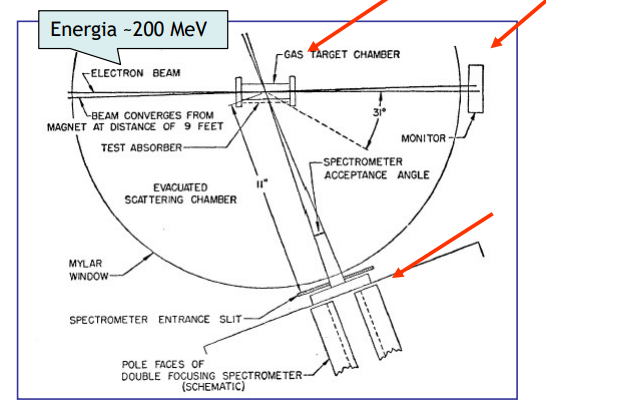
\includegraphics[scale=0.5]{Lezione6/of.png}
  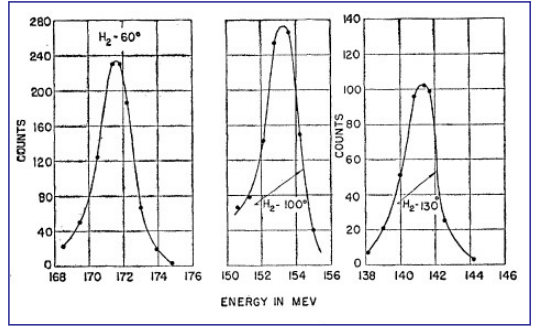
\includegraphics[scale=0.5]{Lezione6/of1.png} 
\end{figure}
L'esperimento di Hofstadter consiste dello studio di collisioni tra elettroni e protone e misuro la sezione d'urto elastica di questo processo. La figura mostra uno schema semplificato della camera di scattering: abbiamo un fascio di elettroni accellerati a $200\,MeV$ quindi ad un'energia che è $400$ volte la loro massa (approssimazione ultra-relativistica esatta). La camera bersaglio è riempita di idrogeno gassoso quindi ci sono tanti protoni. La maggior parte degli elettroni attraverseranno la camera di scattering senza interagire con il bersaglio e vengono misurati dal \textbf{rivelatore monitor} che permette così di misurare il numero di elettronidi ogni impulso. Solo occasionalmente gli elettroni interagiscono nel \textbf{bersaglio} e vengono deflessi a grandi angoli. Gli elettroni deflessi dell'angolo a cui è posto il \textbf{rivelatore} entrano nello spettrometro. Infatti questo rivelatore non si limita a dirmi che sono passati gli elettroni ma mi misura anche l'energia, quindi è uno strumento piuttosto complicato. Per cui lo spettrometro misura la quantità di moto dell'elettrone uscente e quindi ci permette di distinguire lo scattering elastico e anelastico. Dai grafici si vede a diversi angoli in cui posiziono il rivelatore quanti elettroni deviati ho visto e questi eletroni sono anche distribuiti secondo la loro energia. Mi aspetto nel caso di scattering elastico il picco di energia mentre le code rappresentano lo scattering anelastico.
\subsubsection{Risultati per idrogeno}
%IMMAGINE fr
\begin{figure}[htp!]
  \centering
  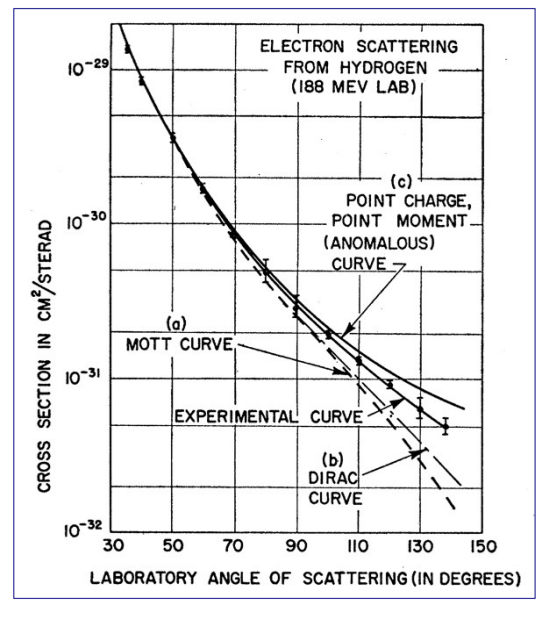
\includegraphics[scale=0.5]{Lezione6/fr.png} 
\end{figure}
Vediamo i risultati di questo esperimento. Vedo quanti elettroni sono stati deviati, quanti elettroni hanno inciso con il bersaglio, so quale è lo spessore del mio bersaglio in quanto so quanto gas ho inserito all'interno della camera, so quanto è grande l'angolo solido di accettanza e quindi posso invertire la formula per la sezione d'urto per misurare la sezione d'urto. Nel grafico si possono vedere diverse curve teoriche, prima però bisogna notare l'asse verticale. Ogni traccia sono circa $20^\circ$. Una tacca sull'asse verticale è molto più importante di una tacca sull'asse orizzontale. Infatti si noti la scala logaritmica sull'asse delle ordinate: dovuto alla singolarità $1/\sin^2{\theta/2}$. Le curve indicate sono: la curva $a)$ è la curva che indica la sezione d'urto di Mott, quindi quella che avrei se il mio bersaglio non avesse spin. La curva $b)$ è un pochino più alta ed è quella di Dirac ed è quando considero anche lo spin del bersaglio (anche il protone ha spin $1/2$). La curva $c)$ è la modifica della curva di Dirac tenendo conto che siamo in presenza di un momento magnetico anomalo e quindi praticamente ad un fattore di forma praticamente uguale a uno. In mezzo ci sono i dati sperimentali che rispetto alla curva puntiforme sono più bassi ed è quello che ci aspettavamo in quanto abbiamo detto che il fattore di forma, che modifica la sezione d'urto perchè sono sensibili alla carica sono sempre minori di uno quindi non fa altro che abbassare. Ricordiamo che il limite di $q^2$ molto piccolo, il limite è circa $1$. Quindi la differenza tra curva puntiforme e curva teorica aumenta con l'aumentare di $q^2$. \textbf{La curva sperimentale indica una correzione:}
\begin{equation*}
    F_1(Q^2)=F_2(Q^2)=1-\frac{Q^2}{r}\langle r_p^2\rangle
\end{equation*} 
con
\begin{equation*}
    \sqrt{\langle r_p^2\rangle}=0.74\pm0.24\,fm
\end{equation*}
\subsubsection{Risultati per particella alpha}
%IMMAGINE tt
\begin{figure}[htp!]
  \centering
  
\includegraphics[scale=0.5]{Lezione6/tt.png} 
\end{figure}
In questo caso il mio bersaglio è la particella $\alpha$. Si vede che la particella $\alpha$ ha spin zero quindi mi confronto con la sezione d'urto di Mott.
\subsubsection{Altri nuclei}
Studi sistematici sui nuclei furono portati avanti dallo stesso Hofstadter aumentando l'energia degli elettroni si può estendere il range di $Q^2$ accessibile. 
\subsection{Il deutone}
Siamo interessati a studiare l'interazione tra due nucleoni partendo dal sistema più semplice studiando il deutone. Fino ad ora abbiamo descritto delle proprietà dei nuclei a partire da osservazioni empiriche che ci hanno portato alla formula di Bethe-Weizs\"acker:
\begin{equation*}
     \text{B.E.}(A,Z)=-a_{1}A+a_{2}A^{\frac{2}{3}}+a_{3}{\frac {Z^2}{A^{\frac{1}{3}}}}+a_{4}{\frac {(N-Z)^{2}}{A}}\pm a_5 A^{-\frac{3}{4}}
\end{equation*}
Descrive parte della fenomenologia osservata: 
\begin{itemize}
    \item interazioni a breve range;
    \item densità uniforme;
    \item bilanciamento tra neutroni e protoni;
    \item energia di "pairing" dei nucleoni che ci spiega perchè certi materiale sono un ottimo combustibile per la fissione oppure no.
\end{itemize}
Questa formula non descrive lo spin ed altri numeri quantci e l'esistenza di strutture nelle energie di legame. Ora vogliamo studiare direttamente l'interazione nucleare. \textbf{Il sistema da cui partire è l'interazione tra due nucleoni.}
\subsubsection{Somma di momenti angolari}
Se abbiamo un'Hamiltoniana invariante per rotazione, il momento angolare totale $\mathbf{J}=\mathbf{L}+\mathbf{S}$ è una quantità conservata, non lo sono invece $\mathbf{L}$ ed $\mathbf{S}$ separatamente mentre $\mathbf{L}^2$ e $\mathbf{S}^2$ si, essendo quantità scalari. Ci si pone il problema di determinare quali sono i valori possibili di $j$ e come sono fatte le funzioni d'onda. La tecnica di base consiste nel fatto che uno classifica le autofunzioni di $\mathbf{L}$ ed $\mathbf{S}$ in base a $j_z=l_z+s_z$ successivamente si usano gli operatori $\mathbf{J}_+=\mathbf{L}_++\mathbf{S}_+$ e $\mathbf{J}_-=\mathbf{L}_-+\mathbf{S}_-$ detti operatori di innalzamento e abbassamento per determinare diverse autofunzoni di $m_j$ per un certo $j$. Utilizzando la relazione (derivata dalle regole di commutazione del momento angolare):
\begin{equation*}
    J_+|j,m_j\rangle=\sqrt{j(j+1)-m_j(m_j+1)}|j,m_j+1\rangle
\end{equation*}
\begin{equation*}
    J_-|j,m_j\rangle=\sqrt{j(j+1)-m_j(m_j-1)}|j,m_j-1\rangle
\end{equation*}
$|j,m_j\rangle$ è la funzione d'onda con momento angolare $j$ e componente $z$ $m_j$. Il risultato è che i possibili valori di $j$ sono $j=l+s,l+s-1,...,|l-s|$.
\subsection{IL sistema del Deutone}
Il deutone è il più semplice stato legato: $N=1$ e $Z=1$. Può essere indicato come $\ch{^2H}$ o $d$ o $D$. La sua massa atomica:
\begin{equation*}
    m(\ch{^2H})=2.014\,101\,778\,120\pm0.000\,000\,000\,122\,u
\end{equation*}
Si nota come questo abbia un eccesso di massa non indifferente noto con una precisione abbastanza grande. Questo ci permette di calcolare la sua energia di legame:
\begin{align*}
B.E.(\ch{^2H})=m(\ch{^2H})-m(\ch{^1H})-m(n)= \\
=2\,u+13.1357217\,MeV \\
-1\,u-7.2889706\,MeV \\
-1\,u-8.0713171\,MeV \\
=-2.224566\,MeV
\end{align*}
Questa è un'energia di legame piccola, infatti si tratta di uno stato molto debolmente legato:
\begin{equation*}
    \frac{B}{A}=1.112283\,MeV
\end{equation*}
Molto minore rispetto al valore tipico di $8\,MeV$. Quindi il legame non è particolarmente forte. La conseguenza di questo fatto è che \textbf{non esistono stati eccitati} il deutone non può e non ha altri livelli energetici al di sotto dello zero. Ha solo questo stato fondamentale. Il raggio dl deutone: $R_d=2.1424\pm0.0021\,fm$. Si noti che il raggio del protone: $R_p=0.8775\pm0.0051\,fm$. Questo significa che il raggio del deutone è maggiore di due volta il raggio del protone. Questo è un altro modo per dire che questo è uno stato legato. L'oggetto ha dimensione più grandi del neutrone e protone presi separatamente. Si possono anche misurare i numeri quantici di questo stato e si scopre che lo spin-parità è $=1^+$ questo significa che il deutone ha parità positiva. Altra proprietà misurata è il momento magnetico del deutone: $\mu_d=0.857438229\pm0.0000000007\,\mu_N$.
\subsubsection{Il deutone: funzione d'onda}
%IMMAGINE pot
\begin{figure}[htp!]
  \centering
  
\includegraphics[scale=0.5]{Lezione6/pot.png} 
\end{figure}
Un primo approccio semplificato, assumiamo il classico potenziale della buca sferica:
\begin{equation*}
    V(r)=\begin{cases} -V_0 & r<R \\ 0 & r>R
\end{cases}
\end{equation*}
Prendiamo il potenziale dato dalla buca sferica, diversamente dal caso del decadimento $\alpha$ non abbiamo una repulsione coulombiana, perchè il neutrone è neutro, e quindi semplicemente non abbiamo il termine che va come $1/r$ ma semplicemente andiamo a zero quando neutrone e protone si staccano. La separazione di variabili dividendo in una parte radiale e l'altra angolare:
\begin{equation*}
    \psi(\mathbf{r})=\frac{u(r)}{r}Y_{l,m}(\theta,\phi)
\end{equation*}
la parte radiale risolve un'equazione agli autovalori:
\begin{equation*}
    -\frac{\hbar^2}{2m}\frac{d^2u}{dr^2}+\left[V(r)+\frac{h^2l(l+1)}{2mr^2}-E\right]u=0
\end{equation*}
Dove $m$ è la massa ridotta. Lo stato di energia minima lo abbiamo per $l=0$ che è il valore che mi minimizza il termine nell'equazione precedente. Quindi ho $Y_{0,0}(\theta,\phi)=\frac{1}{4\pi}$. Se cerco soluzioni per $E<0$ e quindi per stati legati:
\begin{equation*}
    u(r)=\begin{cases} A\sin{k_1r}+B\cos{k_1r}& k_1=\sqrt{\frac{2m(E+V_0)}{\hbar^2}} \quad r<R \\ Ce^{-k_2r}+De^{k_2r} & k_2=\sqrt{\frac{-2mE}{\hbar^2}} \quad r>R
\end{cases}
\end{equation*}
Ovviamente $D=0$ in quanto per far si che la mia funzione d'onda sia normalizzabile non può divergere per $r\to\infty$ e quindi deve essere limitata ed in più per $r\to0$ deve essere continua e quindi $B=0$. Perchè stiamo considerando solo $l=0$? Beh abbiamo visto che esiste un solo stato legato per quanto riguarda il deutone e siccome sappiamo che il sistema di minima energia deve essere $l=0$ (perchè minimizza il potenziale centrale) anche se scopriremo che non è proprio così.

Le condizioni di continuità al bordo della buca:
\begin{equation*}
    A\sin{k_1R}=Ce^{-k_2R} \quad  Ak_1\cos{k_1R}=-Ck_2e^{-k_2R}
\end{equation*}
Facendo il rapporto di queste equazioni si traduce nell'equazione per gli autovalori:
\begin{equation*}
    k_1\cot{k_1R}=-k_2
\end{equation*}
Mettendo dentro i valori visti prima: $R=2.1\,fm$ e l'energia dello stato legato che misuro sperimentalmente $E=-2.2\,MeV$ si può determinare la profondità della barriera di potenziale $V_0=35\,MeV$. La probabilità di trovare un nucleone "fuori" dalla barriera decresce esponenzialmente con una scala di lunghezze:
\begin{equation*}
    \frac{1}{2k_2}=\frac{\hbar}{2\sqrt{-2mE}}=\frac{200\,MeV\,fm}{2\sqrt{938\,MeV\,2,2\,MeV}}=2.2\,fm
\end{equation*}
Quindi abbiamo visto come da una misura di spettroscopia e quindi dalla misura dell'energia di legame la profondità della buca.
\subsubsection{Il deutone: spin e parità }
$\mathbf{J^P}=1^+$. Gli spin dei due nucleoni possono accoppiarsi per dare uno spin totale $S=0$ o $S=1$ (visto che sia il neutrone che il protone hanno spin $1/2$). Il momento angolare totale $J=1$ si può ottenere dalle seguenti combinazioni:
\begin{itemize}
    \item stati $s$: $S=1$, $L=0$;
    \item stati $p$: $S=0$, $L=1$ o $S=1$, $L=1$. Questo perchè il momento angolare totale che ha valore massimo $2$ e valore minimo $0$ in mezzo c'è il valore $1$;
    \item stati $d$: $S=1$, $L=2$
\end{itemize}
La parità dello stato è dato da:
\begin{equation*}
    P(d)=\eta_n\eta_p(-1)^L
\end{equation*}
Con la convenzione usuale degli autovalori di parità $\eta_n=\eta_p=+1$ e quindi solo gli stati $L=0$ e $L=2$ sono permessi visto che abbiamo detto prima che il deutone ha parità positiva. Entrambi gli stati permessi con hanno $S=1$ questo si combina al fatto che abbiamo lo stato fondamentale con $L=0$ e quindi non esiste stato con $J=0$. Quindi non esiste stato legato $0^+$. Possiamo dedurre che \textbf{il potenziale deve dipendere fortemente dallo spin} infatti se combino protone e neutrone a dare spin $=1$ ho lo stato legato. Mentre al contrario se li combino in modo tale da avere spin $=0$ non ho uno stato legato. Nell'atomo di idrogeno questo non succede. Possiamo quindi introdurre dei termini proporzionali a $S^2$ o $\mathbf{s}_1\cdot\mathbf{s}_2$:
\begin{equation*}
    \mathbf{S}^2=(\mathbf{s}_1+\mathbf{s}_2)^2=\mathbf{s}_1^2+\mathbf{s}_2^2+2\mathbf{s}_1\cdot\mathbf{s}_2
\end{equation*}
e quindi 
\begin{equation*}
    \mathbf{s}_1\cdot\mathbf{s}_2=\frac{1}{2}(\mathbf{S}^2-\mathbf{s}_1^2-\mathbf{s}_2^2)=\frac{1}{2}(S(S+1)-s_1(s_1+1)-s_2(s_2+1))\hbar^2
\end{equation*}
\subsubsection{Il deutone: potenziali di tripletto e singoletto}
Di fatto gli spin delle singole particelle sono costanti, è una proprietà del tipo di particella. Dall'ultima relazione per $S=1$:
\begin{equation*}
\mathbf{s}_1\cdot\mathbf{s}_2=\frac{1}{2}(1(1+1)-\frac{1}{2}(\frac{1}{2}+1)-\frac{1}{2}(\frac{1}{2}+1))=\frac{1}{4}
\end{equation*}
Questo implica che questi spin non sono perfettamente allineati. Se lo fossero il loro prodotto scalare sarebbe $\frac{1}{2}$. Per $S=0$:
\begin{equation*}
    \mathbf{s}_1\cdot\mathbf{s}_2=\frac{1}{2}(0(0+1)-\frac{1}{2}(\frac{1}{2}+1)-\frac{1}{2}(\frac{1}{2}+1))=-\frac{3}{4}
\end{equation*}
In questo caso implica che i suoi autovettori siano uno in direzione opposta rispetto all'altro.

Possiamo definire il potenziale separatamente per gli stati di tripletto ($S=1$, $m_s=\pm1,0$) e di singoletto ($S=0$, $m_s=0$):
\begin{equation*}
    V(r)=\left(\mathbf{s}_1\cdot\mathbf{s}_2-\frac{1}{4}\right)V_1(r)+\left(\mathbf{s}_1\cdot\mathbf{s}_2+\frac{3}{4}\right)V_3(r)
\end{equation*}
Si noti che nello stato $L=0$ le coppie $nn$ e $pp$ non possono essere nello stato $S=1$ questa è una conseguenza del principio di esclusione di Pauli. Infatti per fermioni identici la funzione d'onda totale deve essere anti-simmetrica. La simmetria spaziale: $(-1)^l$ e simmetria della componente di spin: $(-1)^{S+1}$. Quindi se abbiamo $L=0$ o $L=2$ la parte spaziale è simmetrica ma d'altra parte abbiamo visto che il potenziale di spin vorrebbe tenermeli allineati. Per avere lo stato legato devo avere il potenziale $V_3(r)$ ma che corrisponde ad una componente di spin simmetrica quindi la mia funzione d'onda simmetrica può funzionare per uno stato $np$ ma non per $nn$ o $pp$. Questo spiega perchè non ci sono nuclei fatti solo di due protoni o solo due neutroni. Posso capire perchè due protoni non possono stare insieme banalmente per la repulsione coulombiana. Ma i due neutroni invece non possono stare insieme semplicemente per una ragione quantistica. La loro funzione d'onda non avrebbe la simmetria giusta.
\subsubsection{Il deutone: momento magnetico}
Il momento magnetico del sistema di spin $S=1$ è dato dalla relazione:
\begin{equation*}
    \bm{\mu}_S=g_S\mu_N\mathbf{S}=g_p\mu_N\mathbf{s}_p+g_n\mu_N\mathbf{s}_n
\end{equation*}
Avevamo visto che $g_p=+5.5857$ e $g_n=-3.8261$. Per calcolare il coefficiente giromagnetico, possiamo proiettare $s_p$ ed $s_n$ sul vettore dello spin totale:
\begin{equation*}
    g_s\mathbf{S}^2=g_p(\mathbf{s}_p\cdot\mathbf{S})+g_n(\mathbf{s}_n\cdot\mathbf{S})=g_p(\mathbf{s}_p^2+\mathbf{s}_p\cdot\mathbf{s}_n)+g_n(\mathbf{s}_n^2+\mathbf{s}_p\cdot\mathbf{s}_n)
\end{equation*}
Sostituendo i valori:
\begin{equation*}
    g_s2=g_p\left(\frac{3}{4}+\frac{1}{4}\right)+g_n\left(\frac{3}{4}+\frac{1}{4}\right)
\end{equation*}
e quindi:
\begin{equation*}
    g_s=\frac{g_p+g_n}{2}=+0.8798
\end{equation*}
Questo è il fattore giromagnetico del deutone nel caso avessi una funzione d'onda con spin $=1$. Il momento magnetico risultante:
\begin{equation*}
    \mu_s=g_s\mu_N=0.8798\mu_N \qquad \mu_d=g_d\mu_N=0.8574\mu_N
\end{equation*}
Si vede come quel valore è vicino ma non uguale a quello misurato sperimentalmente. Questa analisi così semplifica sembra essere effettivamente dominata dalla parte di spin ma c'è qualcosa in più. Per giustificare questa discrepanza la cosa che dobbiamo assumere è che ci sia una parte di momento magnetico non solo dovuta allo spin ma anche dovuta al momento angolare orbitale. Questo ci fa un pochino male in quanto dobbiamo accettare il fatto che non può essere $L$ esattamente $=0$. \textbf{Il deutone allora deve essere in uno stato misto}: $L=0\,+\,L=2$. \textbf{Questo vuol dire che il potenziale di interazione non può essere un potenziale puramente centrale.} Se avessimo un potenziale centrale come quello coulombiano abbiamo visto che $l$ è un buon numero quantico e quindi i miei autostati devono essere in stati con un valore di l ben definito. Se abbiamo un potenziale centrale $l$ è un numero quantico ben definito. Se $l$ non è ben definito perchè siamo obbligati ad invocare uno stato misto che contiene due diversi momenti angolari significa che gli autostati di L non sono autostati dell'Hamiltoniana e quindi l'Hamiltoniana non è centrale. Quindi ci sono delle componenti traversali.
Una distribuzione di cariche in moto, produce un momento magnetico: $\bm{\mu}_l=\frac{q\hbar}{2m}\mathbf{L}$. Nel caso del deutone, $q=e$, $m=2m_N$:
\begin{equation*}
    \bm{\mu}_l=\frac{2\hbar}{4m_N}\mathbf{L}=\frac{1}{2}\mu_N\mathbf{L}
\end{equation*}
Ripetendo lo stesso ragionamento, ma sta volta per la combinazione di $L$ e $S$:
\begin{equation*}
    \bm{\mu}_d=g_d\mu_N\mathbf{J}=\frac{1}{2}\mu_N\mathbf{L}+g_s\mu_N\mathbf{S}
\end{equation*}
Usando:
\begin{equation*}
    \mathbf{J}=\mathbf{L}+\mathbf{S} \qquad \mathbf{L}\cdot\mathbf{S}=\frac{1}{2}\left(\mathbf{J}^2-\mathbf{L}^2-\mathbf{S}^2\right)=\frac{1}{2}(j(j+1)-l(l+1)-s(s+1))\hbar^2
\end{equation*}
La proiezione lungo $J$ dà quindi la relazione:
\begin{equation*}
    g_d\mathbf{J}^2=\frac{1}{2}\mathbf{L}\cdot(\mathbf{L}+\mathbf{S})+g_s\mathbf{S}\cdot(\mathbf{L}+\mathbf{S})
\end{equation*}
Ma quindi:
\begin{equation*}
    g_d=\frac{1}{2}\frac{\mathbf{L}\cdot\mathbf{S}+\mathbf{L}^2}{\mathbf{J}^2}+g_s\frac{\mathbf{L}\cdot\mathbf{S}+\mathbf{S}^2}{\mathbf{J}^2}
\end{equation*}
Allora se $L=0$ allora $g_d=g_s$. Per uno stato con $J=1$, $S=1$, $L=2$ si ottiene:
\begin{equation*}
    g_d=\frac{3}{4}-g_s\frac{1}{2}=0.3101
\end{equation*}
Se lo stato fondamentale è una sovrapposizione degli stati $s$ con $L=0$ e $d$ con $L=2$:
\begin{equation*}
    \psi_d=a_ss+a_dd, \quad |a_s|^2+|a_d|^2=1
\end{equation*}
Il valore di aspettazione del momento magnetico diventa:
\begin{equation*}
    g_d\mu_N=|a_s|^2g_s\mu_N+|a_d|^2\left(\frac{3}{4}-\frac{g_s}{2}\right)\mu_N \quad \Rightarrow\quad 0.8574=|a_s|^20.8798+|a_d|^20.3101
\end{equation*}
\begin{equation*}
    |a_s|^2=0.96 ,\quad |a_d|^2=0.04
\end{equation*}
è un modo per dirmi che queste due componenti sono entrambe diverse da zero. Sono dominato dal fattore con $L=0$ però ho circa un $4\%$ dello stato con $L=2$. Quindi il mio deutone non può essere in uno stato di momento angolare puro.
\subsection{Potenziale tensoriale}
La presenza di una misura di stati $s$ e $d$ indica che il potenziale non può essere puramente centrale: deve comunque essere invariante per rotazioni, dato che il momento angolare totale viene conservato. Spezza il disaccoppiamento tra funzione d'onda di spin ed il momento angolare orbitale che si ha con un potenziale centrale:
\begin{equation*}
    V(r)=\left[\left(\mathbf{s}_1\cdot\mathbf{s}_2-\frac{1}{4}\right)V_1(r)+\left(\mathbf{s}_1\cdot\mathbf{s}_2+\frac{3}{4}\right)V_3(r)\right]+V_T(r)S_{1,2}
\end{equation*}
dove:
\begin{equation*}
    S_{1,2}=3\frac{(\mathbf{s}_1\cdot\mathbf{r})(\mathbf{s}_2\cdot\mathbf{r})}{r^2}-(\mathbf{s}_1\cdot\mathbf{s}_2)
\end{equation*}
La forma di $S_{1,2}$ può avere una spiegazione intuitiva essendo simile alla \textbf{interazione di due momenti magnetici}:
\begin{equation*}
    \mathbf{B}(\mathbf{r})=\frac{\mu_0}{4\pi}\left[\frac{2\mathbf{r(\mathbf{m}\cdot\mathbf{r})}}{r^5}-\frac{\mathbf{m}}{r^3}\right]
\end{equation*}
Campo magnetico generato da un dipolo. E successivamente si può scrivere l'energia potenziale di un dipolo in campo magnetico:
\begin{equation*}
    V(\mathbf{r})=-\mathbf{m}\cdot\mathbf{B}(\mathbf{r})
\end{equation*}
scrivendo i momenti magnetici di neutrone e protone:
\begin{equation*}
    \mathbf{m}_{p,n}=g_{p,n}\mu_N\mathbf{s}_{p,n}
\end{equation*}
si ottiene:
\begin{equation*}
    V_{T}(\mathbf{r})=\frac{\mu_0}{4\pi}\frac{g_pg_n\mu_N^2}{r^3}
\end{equation*}
Questo è un'analogia qualitativa con i dipoli magnetici.
\subsection{Teoria dello scattering}
Qui trattiamo un approccio formalmente esatto al calcolo delle sezioni d'urto che permette di mettere in evidenza alcune proprietà generali di scattering: vedremo quali sono gli stati di momento angolare che contribuiscono alla diffusione e quindi dei limiti alle sezioni d'urto. Il processo logico che seguiremo sarà il seguente: per stati non legati esistono infinite autofunzioni con energia $E$. Una qualunque combinazione lineare di queste è autofunzioni di $E$. Quindi quello che possiamo fare per descrivere l'esperimento è combinare le autofunzione dell'energia in modo tale che descriva un'onda piana incidente ed un'onda diffusa. L'ampiezza di questa onda diffusa sarà al sezione d'urto. Processo più complicato della regola d'oro di fermi. Seguono nelle slide la dimostrazione di autostati di particella libera. 
%\subsection{Interazioni nucleone-nucleone: bassa energia}
\subsection{Sezione d'urto totale}
Per calcolare la sezione d'urto totale dobbiamo integrare s tutto l'angolo solido:
\begin{equation*}
    \sigma=\frac{1}{4k^2}\int d\Omega \left(\sum_{l_1=0}^{\infty}i(2l_1+1)\left[1-e^{2i\delta_{l_1}}\right]P_l(\cos{\theta})\right)^*\left(\sum_{l_2=0}^{\infty}i(2l_2+1)\left[1-e^{2i\delta_{l_2}}\right]P_l(\cos{\theta})\right)
\end{equation*}
Usando la normalizzazione per i polinomi di Legandre.
\begin{equation*}
    \sigma=\frac{\pi}{4k^2}\sum_{l=0}^{\infty}(2l+1)\left|1-e^{2i\delta_l}\right|^2
\end{equation*}
\begin{equation*}
    \sigma=\frac{\pi}{4k^2}\sum_{l=0}^{\infty}(2l+1)\sin^2{\delta_l}
\end{equation*}
La sezione d'urto risulta scomposta in sezioni d'urto parziali. Abbiamo visto che la sezione d'urto differenziale è complicata perchè ha vari termini di interferenza quando andiamo a vedere la sezione d'urto totale grazie alla proprietà dei polinomi di Legendre possiamo sommare le varie sezioni d'urto per $l = 0,1,2,\ldots$. \textbf{La sezione d'urto parziale è limitata}: cioè ogni termine in questa somma siccome c'è il $\sin^2{\delta_l}$ non può mai essere maggiore di quando il $\sin^2{\delta_l}=1$. Quindi abbiamo:
\begin{equation*}
    \sigma\le\frac{4\pi(2l+1)}{k^2}
\end{equation*}
Da qui mi verrebbe da dire: ok la sezione d'urto parziale è limitata superiormente ma ho una sommatoria infinita.
\subsection{Parametro di impatto}
Sembrerebbe che il calcolo delle sezioni d'urto richieda una sommatoria infinita. In realtà alla sezione d'urto reale contribuiscono solo un numero limitato di onde parziali. Una particella con momento $p=\hbar k$ e momento angolare $L^2=l(l+1)\hbar^2$, passerà tipicamente ad una distanza $b$.
%IMMAGINE yt
\begin{figure}[htp!]
  \centering
  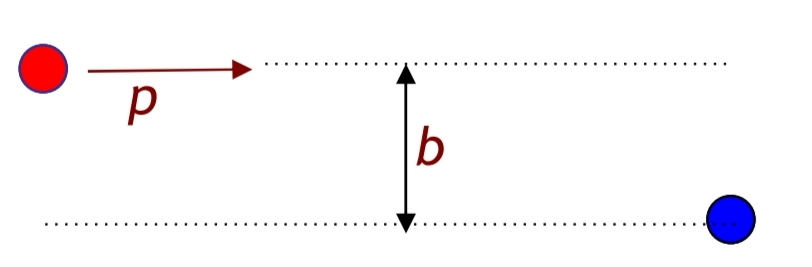
\includegraphics[scale=0.3]{Lezione6/yt.jpg} 
\end{figure}
Se il potenziale si estende fino ad un raggio $R$, influenza gli stati di momento angolare fino a: $l\hbar=pR\to l=kR$ perchè momenti angolari più grandi, parametri di impatto grandi (più grande di $R$ e che quindi la particella passa fuori dal nucleo). Ho qualcosa di fisico che mi dice: se io ho un nucleo e un potenziale con una certa estensione quando vado fuori da questa estensione il mio momento angolare sarà limitato da $pR$ e quindi il momento angolare totale avrà un valore massimo $l\hbar=pR$. Questo equivale a dire che il numero quantico del momento angolare è limitato. Quindi il numero di onde parziali da considerare aumenta con l'energia. Questo perchè $R$ è fissato dal potenziale mentre $k$ aumenta con l'energia. Tuttavia abbiamo una limitazione sulla sezione d'urto parziale. Quindi abbiamo una limitazione sulla sezione d'urto totale:
\begin{equation*}
        \sigma\le\frac{4\pi}{k^2}\sum_{l=0}^{kR}(2l+1)=\frac{4\pi}{k^2}(kR+1)^2=4\pi\left(R+\frac{1}{k}\right)^2=4\pi(R+\lambda)^2
\end{equation*}
Dove la somma dei numeri dispari può essere vista come l'area di un quadrato e $\lambda$ è la \textbf{lunghezza d'onda di De Broglie} è la lunghezza d'onda dell'autofunzione della mia particella. Quindi la mia particella ha una sezione d'urto che ha un valore massimo che è un cerchio di raggio pari all'interazione del potenziale più la lunghezza d'onda di De Broglie. Classicamente uno si aspetta che il raggio dell'interazione sarebbe dovuto essere il limite superiore. Invece grazie alla meccanica quantistica non è così. Abbiamo un termine ulteriore. Questa cosa è importante in un caso già visto. Se ci si pensa bene quando abbiamo visto le sezione d'urto per fissione abbiamo visto che i nuclei con $A=200$ avevano un raggio di circa $7\,fm$ o $8\,fm$. Per cui la dimensione del nucleo su cui andava a sbattere il neutrone è qualcosa come un dischetto di $50\,fm^2\approx0.5\,b$ mentre invece abbiamo visto le sezione d'urto sono dell'ordine di centinaia di barn. In più abbiamo visto che aumentava con il diminuire dell'energia dei neutroni. Man mano che l'energia diminuisce, la lunghezza d'onda del neutrone aumenta (è come se fosse più grande) e quindi ha maggiori possibilità di interagire.
\subsection{Interazioni nucleone-nucleone: bassa energia}
Si dimostra che per $k$ che tende a zero la sezione d'urto tende ad un valore costante. E con $k$ che tende a zero c'è solo scattering con momento angolare $=0$. Infatti a basse enegie contribuiscono solo collisioni con momento orbitale $L=0$. La sezione d'urto è approssimativamente indipendente dall'angolo solido. Quindi diventa una sezione d'urto isotropa. Questa è una giustificazione a posteriori del fatto che nella fissione nucleare dove il neutrone dopo aver compiuto una collisione viene scatterato a caso (infatti vengono fatte a basso momento) e quindi ho scattering isotropo. Misurando la sezione d'urto in funzione dell'energia verifico effettivamente questo andamento:
%IMMAGINE uu
\begin{figure}[htp!]
  \centering
  
\includegraphics[scale=0.16]{Lezione6/uu.png} 
\end{figure}
La cosa importante che la lunghezza di scattering di $nn$ o $np$ o $pp$ si ottiene che i valori di lunghezza di scattering sono compatibili. Quindi le interazioni forti sono indipendenti dalla carica elettrica. Quindi agli occhi delle interazioni forti i neutroni e i protoni sono praticamente indistinguibili. \textbf{Le interazioni forti sono indipendenti dalla carica}.
\subsection{Core repulsivo in interazioni tra nucleoni}
La lunghezza di scattering da anche informazioni sul potenziale. Per una particella libera il $kR$ quindi la fase della mia onda sferica cresce in maniera uguale sia dentro che fuori dal nucleo. Quindi la mia funzione d'onda è esattamente una sinusoide. Se invece ho una buca di potenziale attrattiva (potenziale negativo) ho un'energia cinetica maggiore all'interno del nucleo quindi la funzione d'onda oscilla più velocemente all'interno del nucleo. Quando esco inizio ad oscillare più lentamente ma l'oscillazione veloce precedente mi ha dato uno sfasamento positivo. Viceversa se avessi un potenziale repulsivo quindi una buca di potenziale alta. Dentro la buca di potenziale la funzione d'onda oscilla più lentamente quindi quando esce dalla buca avrà fatto meno "strada" e mi ritroverò con uno sfasamento negativo. Quindi lo sfasamento ci dà un'informazione se il potenziale è attrattivo o repulsivo (se minore di zero o maggiore di zero). 

Quello che si vede nel secondo grafico è presente lo sfasamento in funzione dell'energia del neutrone che viene fatto collidere con il protone. Lo sfasamento cambia segno se vano in alte energie (equivalente ad avere Q valore grande quindi si possono misurare distanze piccole) quello che vedo è che lo sfasamento è negativo. A basse energie se sto  guardando un oggetto con una lunghezza d'onda grande (con dimensioni maggiori) il mio sfasamento è positivo. Quindi quello che vedo è che ho una transizione tra un potenziale attrattivo nel complesso a grandi distanze ma se vado molto vicino al centro di forze inizio a vedere un core repulsivo che mi tende a buttare fuori i miei nucleoni e a non formare uno stato legato. Questo core repulsivo è quello che ci spiega perchè quando costruiamo i nuclei abbiamo una densità costante. I neutroni non li possiamo mettere vicini quanto vogliamo ma quando li avviciniamo dopo un po' si fermano. 
%IMMAGINE ii
\begin{figure}[htp!]
  \centering
  
\includegraphics[scale=0.13]{Lezione6/ii.jpg} 
\end{figure}
\subsection{Interazione Spin-Orbita}
%IMMAGINE oo
\begin{figure}[htp!]
  \centering
  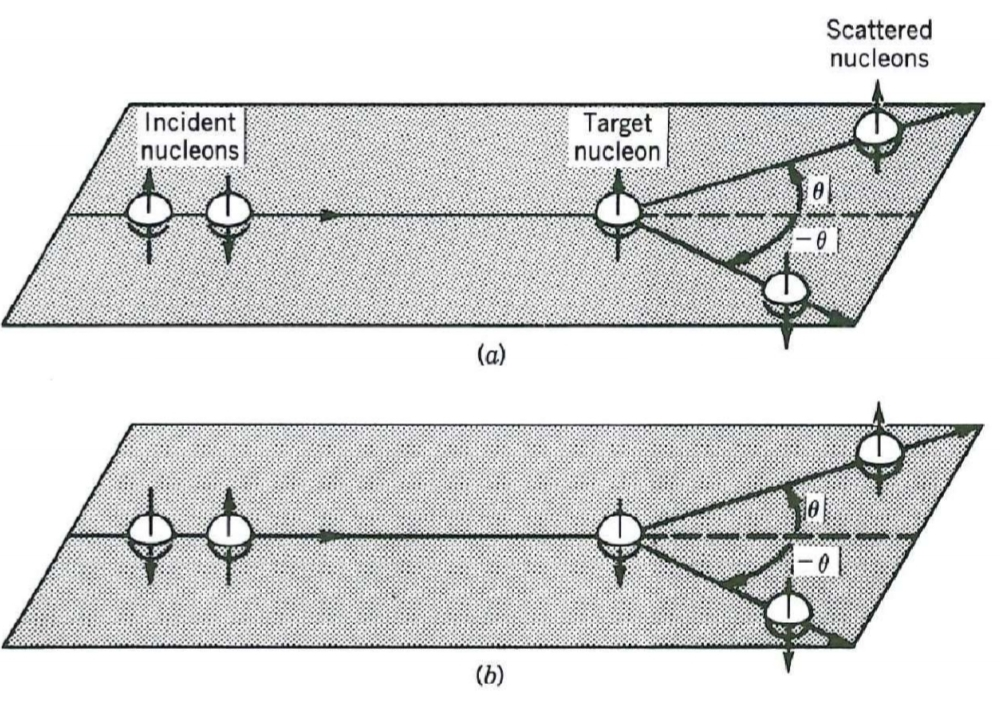
\includegraphics[scale=0.14]{Lezione6/oo.jpg} 
\end{figure}
Succede qualcosa di strano: supponiamo di avere un fascio di nucleoni che non sono polarizzati. Hanno spin alcuni su alcuni giù. Li mando contro un bersaglio che presenta un'orentazione non ben definita. Quello che succede vado a vedere i nucleoni che sono stati deviati a destra e i nucleoni che sono stati deviati a sinistra. Mi rendo conto che il primo gruppo ha uno spin preferenziale mentre il secondo quello opposto. Quindi parto da uno stato senza nessun tipo di polarizzazione finisco in uno stato in cui i due gruppi hanno una direzione preferita. Quindi come risultato si osserva una \textbf{polarizzazione} dei nucleoni uscenti:
\begin{equation*}
    P(\theta)=\frac{N_{\uparrow}(\theta)-N_{\downarrow}(\theta)}{N_{\uparrow}(\theta)+N_{\downarrow}(\theta)}
\end{equation*}
Si può descrivere tramite un potenziale del tipo:
\begin{equation*}
    V_{SO}\mathbf{S}\cdot(\mathbf{r}\times\mathbf{p})=V_{SO}\mathbf{S}\cdot\mathbf{L}
\end{equation*}
è detta interazione spin-orbita perchè è un'interazione tra il momento angolare orbitale e il momento angolare di spin. Come possiamo giustificare questa cosa? Come mai si crea questa asimmetria? Consideriamo il caso in cui ho il nucleo bersaglio e due protoni come in figura. Assumiamo che $V_{SO}(r)$ si attrattivo (ovvero abbia un segno meno). e supponiamo che i due nucleoni abbiamo spin uscente dalla pagina. Per il primo nucleone, $\mathbf{S}\cdot\mathbf{L}<0$: la forza diventa repulsiva.

Viceversa per il secondo nucleone $\mathbf{S}\cdot\mathbf{L}>0$: la forza rimane attrattiva.
%IMMAGINE kk
\begin{figure}[htp!]
  \centering
  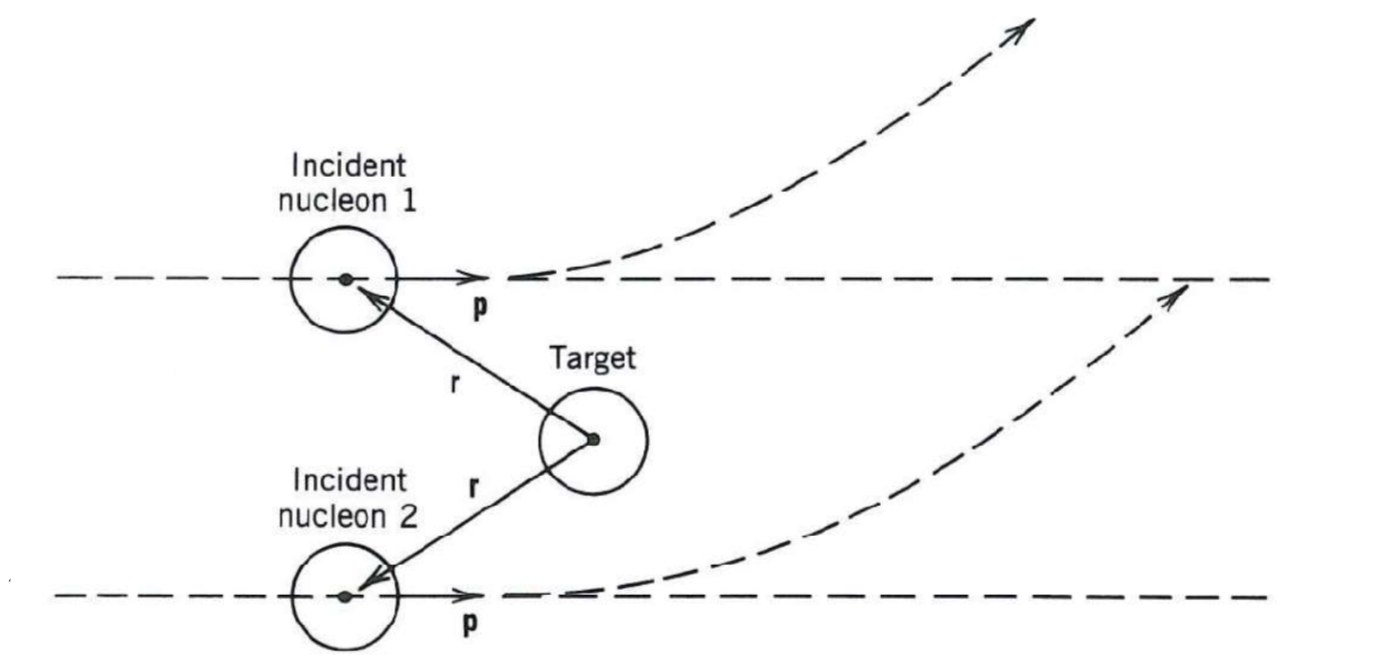
\includegraphics[scale=0.14]{Lezione6/kk.png} 
\end{figure}
\subsection{Scattering nucleone-nucleone: forza di scambio}
%IMMAGINE hh
\begin{figure}[htp!]
  \centering
  
\includegraphics[scale=0.14]{Lezione6/hh.png} 
\end{figure}
L'ultimo concetto è che quando facciamo interagire due particelle ci aspettiamo che all'aumentare della quantità di moto l'interazione (o la deflessione) diventi molto più debole. Classicamente ci aspettiamo che l'ordine di grandezza della deflessione sia:
\begin{equation*}
    \theta=\frac{\Delta p}{p}=\frac{F\Delta t}{p}=\frac{(V_0/R)(R/v)}{p}=\frac{V_0}{2(\frac{1}{2}mv^2)}
\end{equation*}
Quindi mi aspetto (come potevo immaginare) che all'aumentare dell'energia l'angolo di deflessione diminuisce. Ad asempio a $500\,MeV$ ci aspettiamo circa $2^\circ$. Quindi ci aspettiamo che la sezione d'urto sia piccata ad angoli piccoli e poi decresca man mano a deflessioni maggiori. Quello che si vede invece è che a piccoli angoli ho comunque una sezione d'urto grande. C'è il calo all'aumentare dell'angolo ma a grandi angoli ho un'altra risalita:
%IMMAGINE lop
\begin{figure}[htp!]
  \centering
  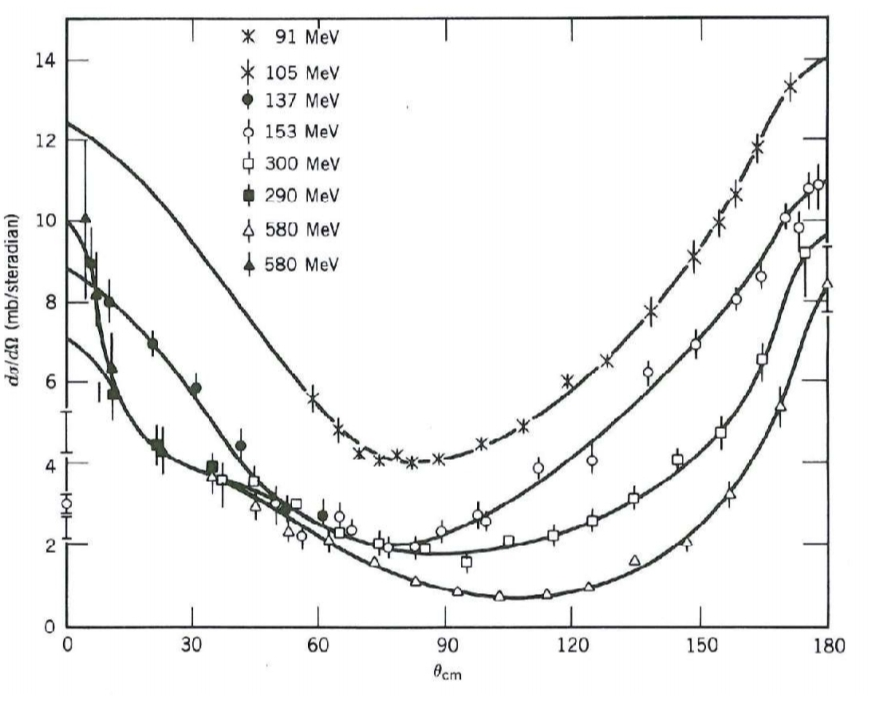
\includegraphics[scale=0.2]{Lezione6/lop.jpg} 
\end{figure}
Ho una probabilità molto grande che il neutrone torni indietro (sezione d'urto alta a $180^\circ$). Questo ha portato alla formulazione di una nuova ipotesi di interazione, \textbf{Interazione di scambio}: l'interazione (la forza) è mediata dallo scambio di particelle. In particolare in questo modello possiamo spiegare l'osservazione che l'interazione sia mediata dallo scambio di una particella carica. Ovvero il mio protone e neutrone si avvicinano ma quello che succede è che il protone si trasformi in un neutrone ed emette una particella di carica positiva che colpisce il neutrone, gli trasferisce un momento e lo trasforma in un protone. Per cui quello che vedo in uscita non è altro che il protone che torna indietro. Quel protone ovviamente non è quello iniziale ma il neutrone trasformato in protone. 

Questo è un punto importante perchè la particella in questione non può venir prodotta realmente: violerebbe la conservazione di energia e momento. Tuttavia è permessa dal principio di indeterminazione: $\Delta E\Delta t>\hbar$ ci dice che per processi di durata $\Delta t$ non possiamo verificare la conservazione dell'energia a meno di $\Delta E>\hbar/\Delta t$. Per scambiare interazioni nucleari il mediatore ha bisogno di coprire almeno una distanza $r_0$ corrispondente a $\Delta t\sim r_0/c$. Quindi è possibile avere masse:
\begin{equation*}
    m_Xc^2<\hbar/\Delta t=\hbar c/r_0\sim200\,MeV
\end{equation*}
Una forma usata del potenziale di interazione:
\begin{equation*}
V(r)=\frac{g_\pi^2m_X}{3}\left[\mathbf{s}_1\cdot\mathbf{s}_2+S_{1,2}\left(1+\frac{3R}{r}+\frac{3R^2}{r^2}\right)\right]\frac{e^{-r/R}}{r/R}
\end{equation*}
In questa formula quindi ho: un termine che dipende dallo spin (il prodotto scalare). Questo termine mi porta ad allineare lo spin di protone e neutrone. Un termine tensoriale che viola la forma centrale del potenziale. Ed infine per definire l'interazione ci metto dentro che mi descrive il range dell'interazione (il range del potenziale) quindi una diminuizione esponenziale che dipende da $R$ che è il range del potenziale. Ci metto qua dentro il termine di massa che è collegato alla dimensione dell'interazione.
\begin{equation*}
    S_{1,2}=3\frac{(\mathbf{s}_1\cdot\mathbf{r})(\mathbf{s}_2\cdot\mathbf{r})}{r^2}-(\mathbf{s}_1\cdot\mathbf{s}_2)\qquad R=\frac{\hbar}{m_Xc}
\end{equation*}